\documentclass[tikz,
               border=3mm]{standalone}
\begin{document}
    \begin{tikzpicture}
\draw (-15,0) -- (15,0);
\foreach \i/\o/\r in {0/0/\pm0.0,1/1/0.25,2/2/0.5,3/3/0.75,4/4/1.0,5/5/1.25,6/6/1.5,7/7/1.75,8/8/2.0,9/9/2.5,10/10/3.0,11/11/3.5,12/12/\infty,13/nan/nan,14/nan/nan,15/nan/nan,-1/-1/-0.25,-2/-2/-0.5,-3/-3/-0.75,-4/-4/-1.0,-5/-5/-1.25,-6/-6/-1.5,-7/-7/-1.75,-8/-8/-2.0,-9/-9/-2.5,-10/-10/-3.0,-11/-11/-3.5,-12/-12/-\infty,-13/nan/nan,-14/nan/nan,-15/nan/nan}
{
\draw (\i,0.1) -- + (0,-0.2) node[below] {$\o$} + (0,0.0) node[above] {$\r$};
}
%\foreach \i in {0.5, 0.7, 0.9}% points on line
%\fill[red]  (\i,0) circle (0.6 mm);
    \end{tikzpicture}
\end{document}